\documentclass{report}
\usepackage[utf8]{inputenc}
\usepackage{amssymb}
\usepackage{amsmath}
\usepackage{hyperref}
\usepackage{tcolorbox}
\tcbuselibrary{theorems}
\usepackage{physics}
\usepackage{graphicx}


% Things I use, but too lazy to find how again

%%%%%%%%%%%%%%%%%%%%%%%%%%%%%%%%%%%%%%%%%%%%%%%%%%%%
% Make a hyperlink to another section:
% \hyperref[sec:hello]{Word of text} (set link to hello)

% \section{Hello World} 
% \label{sec:hello} (define a label for the section
%%%%%%%%%%%%%%%%%%%%%%%%%%%%%%%%%%%%%%%%%%%%%%%%%%%%
% Make an unordered list:
% \begin{itemize}
%   \item 
%   \item
% \end{itemize}
%%%%%%%%%%%%%%%%%%%%%%%%%%%%%%%%%%%%%%%%%%%%%%%%%%%%
% Make an ordered list:
% \begin{enumerate}
%   \item 
%   \item
% \end{itemize}
%%%%%%%%%%%%%%%%%%%%%%%%%%%%%%%%%%%%%%%%%%%%%%%%%%%%
% Make a matrix
%\begin{bmatrix}
%        x_1y_1 & x_1y_2 & \dots  & x_1y_m \\
%        x_2y_1 & x_2y_2 & \dots  & x_2y_m \\
%        \vdots & \vdots & \ddots & \vdots \\
%        x_ny_1 & a_{m2} & \dots  & x_ny_m \\
%   \end{bmatrix}
%%%%%%%%%%%%%%%%%%%%%%%%%%%%%%%%%%%%%%%%%%%%%%%%%%%%
% Make an equation:
% \begin{equation}
% ...
% \end{equation}
%%%%%%%%%%%%%%%%%%%%%%%%%%%%%%%%%%%%%%%%%%%%%%%%%%%%
% Theorems:
%\begin{mytheo}{Title}{NameOfTheorem}
% ...
%\end{mytheo}
%%%%%%%%%%%%%%%%%%%%%%%%%%%%%%%%%%%%%%%%%%%%%%%%%%%%
% N'th order linear equation
% $$y^{(n)}(t) + ... + p_1(t)y'(t) + p_0(t)y(t) = 0$$
%%%%%%%%%%%%%%%%%%%%%%%%%%%%%%%%%%%%%%%%%%%%%%%%%%%%

\newtcbtheorem[number within=section]{mytheo}{}
{colback=orange!5,colframe=green!35!black,fonttitle=\bfseries}{th}

\hypersetup{
    pdftitle={Mechanics},
    pdfpagemode=FullScreen,
}




\title{Mechanics}
\author{Arun Khanna}
\date{}

\begin{document}

\maketitle
\tableofcontents

\chapter{Linear Motion and Kinematics of Point Mass}
\section{Displacement, Velocity and Acceleration}
\subsection{Displacement}
Let's get started with some basic definitions.
\begin{mytheo}{Displacement}{disp}
    Displacement is simply a measure of how much an object's position changes.
    
    It is denoted by $\Delta x$ and has S.I. units in [m]
\end{mytheo}

This is not the same thing as distance travelled! Displacement is the same thing as taking a snapshot before and after some time interval and seeing how much the position of an object changed. It has a direction $+$ if it goes in the direction of an axis we define and $-$ otherwise

The following image may help understand it better:

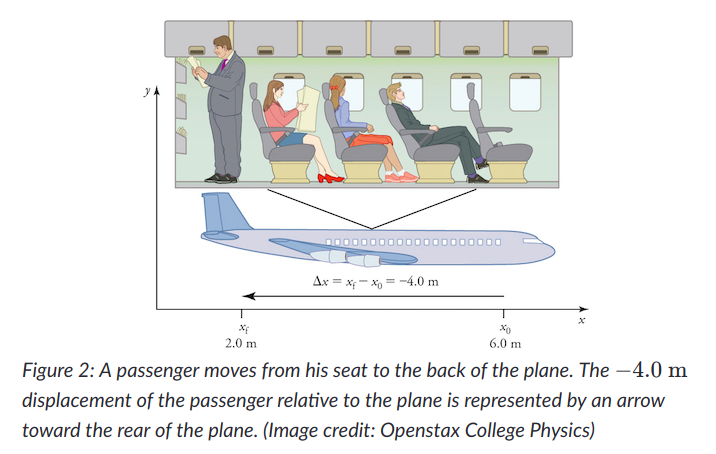
\includegraphics[scale=0.5]{displacement.png}

\subsection{Velocity}

\begin{mytheo}{Average Velocity}{vel}
    Average velocity is the rate of change of the position of an object with respect to time.
    
    It is denoted by $v$ and has S.I. units in [m/s]
\end{mytheo}

This is just a measure of how "fast" something is going.


As we decrease the time interval we're considering, we can get finer and finer linear approximation to the velocity. We call this value the instantaneous velocity.

\begin{mytheo}{Instantaneous Velocity}{instVel}
    Instantaneous Velocity is the limiting value of $\Delta x / \Delta t$ as $\Delta t$ approaches 0
    
    $$\va{v} = \lim_{\Delta t \to 0}\frac{\Delta x}{\Delta t} = \dv{x}{t}$$
\end{mytheo}

This is usually what we will mean when we describe velocity.

If we graph position and time in a graph, the slope of a tangent line at any particular point will in fact be the velocity at that point.

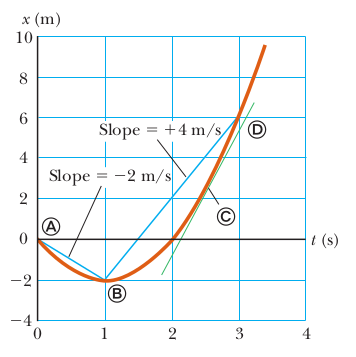
\includegraphics[scale=0.5]{velocity.png}


An important thing to note about velocity is that it has a direction as well as a magnitude. When we describe the speed of some object, we need to know in which direction (left, right, etc.) it's going in to know the velocity.


\subsection{Acceleration}

\begin{mytheo}{Acceleration}{acc}
    Acceleration is a measure of how much the \textbf{velocity} of an object over time. 
    
    $$a = \lim_{\Delta t \to 0}\frac{\Delta v}{\Delta t} = \dv{v}{t}=\dv[2]{x}{t}$$
    
    It's SI units are $[m/s^2]$
\end{mytheo}

There must be an acceleration even when we keep a constant speed, but change direction since acceleration measures change in velocity and velocity depends on direction as well as speed.





\section{Kinematics Equations}
The Kinematics Equations help us relate the following quantities:
\begin{itemize}
    \item $\Delta x$ - Displacement
    \item $\Delta t$ - Time
    \item $v_0$ - Inital Velocity
    \item $v_f$ - Final Velocity
    \item $a$ - Constant Acceleration
\end{itemize}

under constant acceleration. 

The equations are:
\begin{mytheo}{Kinematics Equations}{kin}
    The Kinematics Equations each are missing one variable:
    $$v_f-v_i = a\Delta t \text{  (Missing }\Delta x \text{)}$$
    $$\Delta x = \left( \frac{v_f+v_i}{2}\right)\Delta t \text{  (Missing } t \text{)}$$
    $$\Delta x = v_0\Delta t + \frac{1}{2}a(\Delta t)^2 \text{  (Missing } v_f \text{)} $$
    $$v_f^2-v_i^2 = 2a\Delta x \text{(Missing } \Delta t \text{)}$$
\end{mytheo}

\hyperref[sec:kin]{The proofs are in the appendix.}

\section{Two and More Dimensions of Motion}
To analyze motion in multiple dimensions, we can simply break down the motion into one dimensional components using some orthogonal basis.

After breaking the motion apart, we can then apply what we know about motion in one dimension to each component of motion.

Take for example a projectile. It may initially seem complicated, however, when we break down the motion we see that it is simply acceleration from gravity in one direction (downwards):

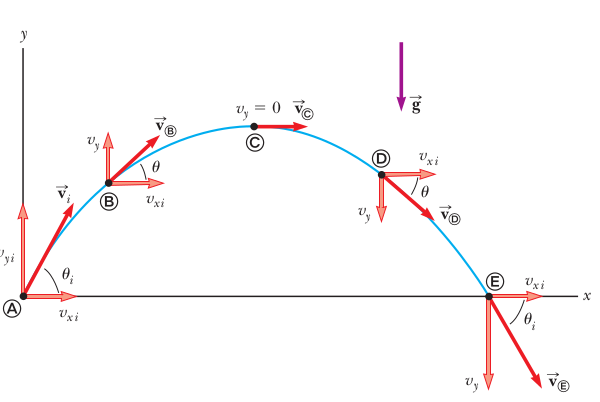
\includegraphics[scale=0.4]{proj.png}


\section{Newton's Laws of Motion}

What is a force? A force can be seen as a push or pull of some point mass. There are two main kinds of forces:
\begin{itemize}
    \item \textbf{Contact Forces}: Contact forces are forces that need to make contact in order to do something.
    \item \textbf{Field Forces}: Field forces do not need to make contact to do something. Think about gravity or electrostatic attraction and repulsion. 
\end{itemize}

Forces are in fact vectors, they have both a magnitude and direction. Intuitively, this makes sense, gravity both has some magnitude and points downwards.

\subsection{Newton's First Law}

\begin{mytheo}{Newton's First Law}{newFirst}
    An object moving with constant velocity in one direction will continue to do so, unless it is acted upon by an outside force.
\end{mytheo}

This also is true for a velocity of 0, if an object is at rest it will stay at rest unless acted upon by another body,

Another way of phrasing Newton's First Law is:

\begin{mytheo}{Alternative Phrasing of Newton's First Law}{altNewFirst}
    It is always possible to find a inertial reference frame such that an object has a constant velocity if the object is not being acted on by external forces.
\end{mytheo}

\subsection{Newton's Second Law}
Before discussing Newton's Second Law, let's first desribe a quantity that almost everyone is familiar with, \textbf{mass}.

What is mass? Why do we call a rock more massive than, for example, a feather?

\begin{mytheo}{Mass}{mass}
    Mass is defined to be the resistance of an object to changes in velocity. It is in fact, an inherent property of the object and is independent of its surroundings
\end{mytheo}

It turns out that through experimentation that when we apply a constant force to an two objects of different masses, the acceleration of the objects are inversely proportional to the masses:

$$\frac{m_2}{m_1} = \frac{a_1}{a_2}$$

This brings us to Newton's second law:

\begin{mytheo}{Newton's Second Law}{newSecond}
    If we are in an inertial frame of reference, the sum of the forces of an object of constant mass is:
    $$\sum \mathbf{F} = m\mathbf{a}$$
\end{mytheo}

This is only true when we're going at a speed far slower than that of light (things become weird when we go around that speed).

\subsection{Newton's Third Law}

Newton's Third Law is relatively straightforward:

\begin{mytheo}{Newton's Third Law}{newThird}
    If a force is exerted by object 1 on object 2 $\mathbf{F_{12}}$, then a force of equal magnitude but in the opposite direction will be exerted by object 2 on object 1 $\mathbf{F_{21}}$:
    
    $\mathbf{F_{21}}$ = -$\mathbf{F_{12}}$
\end{mytheo}


This is the why we are balanced on the ground even though we are feeling the force of gravity downwards on us. There is a contact force, called the $normal force$, that exerts a force equivalent to that exerted by gravity on us.






\section{Linear Momentum, Impulse and Conservation of Linear Momentum}


We see that the derivative of the sum of $m_i\mathbf{v_i}$ is in fact constant. What is this quantity?

We call this \textbf{momentum}:

\begin{mytheo}{Linear Momentum}{linMom}
    Linear momentum of a point mass is defined to be the product of the mass and velocity:
    
    $$\mathbf{p} = m\mathbf{v}$$
    
\end{mytheo}


\subsection{Forces and Momentum}

From Newton's 2nd Law, we know that:

$$\sum \mathbf{F} = \mathbf{F_{net}} = m\mathbf{a}$$
$$\mathbf{F_{net}} = m\dv{\mathbf{v}}{t} = \dv{(m\mathbf{v})}{t}$$

Thus, for the case of constant mass, it turns out that the net force on an object is just the time derivative of momentum!

It turns out that this is true even when the mass is in fact changing! This is in fact the most general form of Newton's second law:

\begin{mytheo}{General Version of Newton's 2nd law}{genNewSec}
    The net force on an object is just the time derivative of momentum:
    $$\sum \mathbf{F} = \mathbf{F_{net}} = \dv{\mathbf{p}}{t} $$
\end{mytheo}

Let's rewrite this in integral form:

$$\int_{t_0}^{t_f}\mathbf{F_{net}}\dd t = \int_{t_0}^{t_f}\dd \mathbf{p} $$

$$\int_{t_0}^{t_f}\mathbf{F_{net}}\dd t = \mathbf{p_f} - \mathbf{p_i} = \Delta \mathbf{p}$$


Thus, applying a force over some time interval will change the momentum. This change is called impulse:

\begin{mytheo}{Impulse}{impulse}
    Impulse is the integral of force with respect to some time interval:
    $$\mathbf{J} = \int_{t_0}^{t_f}\mathbf{F_{net}}\dd t$$
\end{mytheo}

This gives us the momentum-impulse theorem:
\begin{mytheo}{Momentum-Impulse Theorem}{momImp}
    The change of momentum of an object is equal to the impulse applied to that object:
    
    $$\Delta \mathbf{p} = \mathbf{J} = \int_{t_0}^{t_f}\mathbf{F_{net}}\dd t$$
    
\end{mytheo}

\subsubsection{Momentum of System of Particles}

Consider $k$ particles with differing masses and velocities.

We define the total momentum of this system to be the vector sum of the individual momentum of the k particles:

$$\mathbf{p_{tot}} = \mathbf{p_1} + \dots + \mathbf{p_k} = \sum_1^k m_i\mathbf{v_i}$$

In addition, say that we apply $k$ different forces on each of the particles. The total force is:

$$\mathbf{F_{tot}} = \mathbf{F_1} + \dots + \mathbf{F_k}$$

If these are the only forces on each of the particles, then we can use the general version of Newton's 2nd Law:

$$\mathbf{F_{tot}} = \dv{\mathbf{p_1}}{t} + \dots + \dv{\mathbf{p_k}}{t}$$
$$=\dv{(\mathbf{p_1} + \dots + \mathbf{p_k})}{t} = \dv{\mathbf{p_{tot}}}{t}$$

Thus:

\begin{mytheo}{Applying force to System of Particles}{forceSys}
    Applying a total force of $\mathbf{F_{tot}}$ to a system of particles (where the individual forces applied to each particle can in fact be different) is equal to the total change in momentum of the system:
    $$\mathbf{F_{tot}} =\dv{\mathbf{p_{tot}}}{t}$$
    $$\int_{t_i}^{t_f}\mathbf{F_{tot}} = \Delta\mathbf{p_{tot}}$$
    where for $k$ particles:
    $$\mathbf{F_{tot}} = \mathbf{F_1} + \dots + \mathbf{F_k}$$
    $$\mathbf{p_{tot}} = \mathbf{p_1} + \dots + \mathbf{p_k}$$

\end{mytheo}

\subsection{Conservation of Angular Momentum}
Say we have an object $A$ exerting a force on another object $B$.
We know that from Newton's 3rd law that:

$$\mathbf{F_{AB}} = -\mathbf{F_{BA}}$$

Rearranging terms, we get:
$$\mathbf{F_{AB}} + \mathbf{F_{BA}} = \mathbf{0}$$

Let's also suppose there are no external forces acting in our system. Thus the only force on $A$ is from $B$ and vice versa. Thus, from Newton's 2nd Law:

$$\sum \mathbf{F_A} = \mathbf{F_{BA}} = m_A\mathbf{a_A}$$
$$\sum \mathbf{F_B} = \mathbf{F_{AB}} = m_B\mathbf{a_B}$$

Plugging these into our original equation:

$$m_B\mathbf{a_B} + m_A\mathbf{a_A} = \mathbf{0}$$

We know that acceleration is the time derivative of velocity. Thus,

$$m_A\dv{\mathbf{v_A}}{t} + m_B\dv{\mathbf{v_B}}{t} = \mathbf{0}$$

Using the property of linearity of differentials:

$$\dv{(m_A\mathbf{v_A} + m_B\mathbf{v_B})}{t} = 0$$

This means that the quantity 
$(m_A\mathbf{v_A} + m_B\mathbf{v_B})$ must in fact be constant!

If we have multiple objects in a system with no external forces, we can make a similar analysis to each pair of objects to conclude
Thus:
\begin{mytheo}{Conservation of Momentum}{consMom}
    In the absence of external forces on a system of particles, the total momentum of a system is constant
\end{mytheo}


\section{Uniform Circular Motion}
Let's discuss the case when we have an object moving in a circle at constant speed.

Note that the speed is constant, but the velocity is constantly changing, meaning there must be some force that is involved. 

Consider the following image:


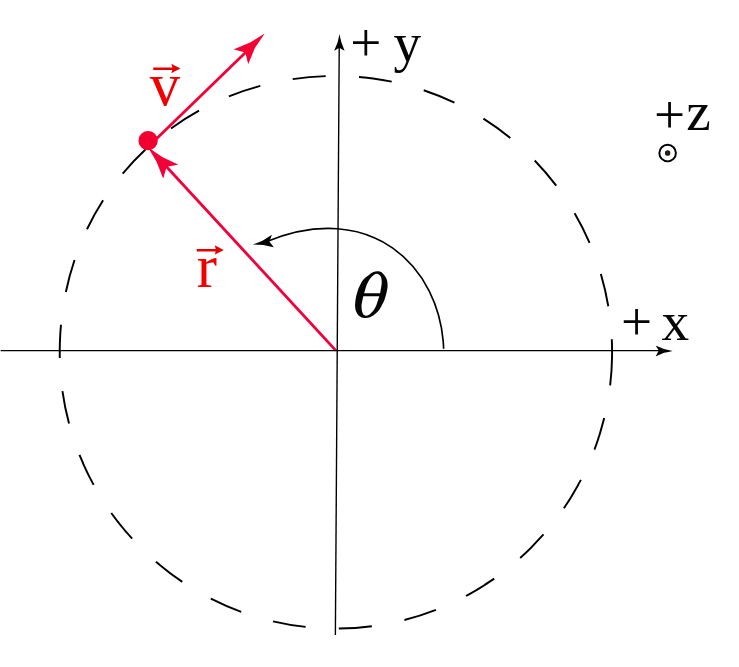
\includegraphics[scale=0.3]{circular_motion.png}


The position vector as a function of the angle $\theta$ is given by:

$$\mathbf{r}(\theta) = R(\cos(\theta)\hat{i} + \sin(\theta)\hat{j})$$

Taking the derivative of this expression with respect to time gives us the velocity vector:

$$\mathbf{v}(\theta) = \dv{\mathbf{r}(\theta)}{t} = R\left(\dv{\cos(\theta)}{t}\hat{i}+\dv{\sin(\theta)}{t}\hat{j}\right)$$

Using the chain rule,

$$\mathbf{v}(\theta) = R(-\sin(\theta)\dv{\theta}{t}\hat{i}+\cos{(\theta)}\dv{\theta}{t}\hat{j})=R\dv{\theta}{t} \left(-\sin(\theta)\hat{i}+\cos{(\theta)}\hat{j}\right)$$

Notice that this is in fact perpendicular to the position vector!

Now to find the acceleration, or the rate at which the velocity vector is changing, we can take another derivative:

$$\mathbf{a}(\theta) = \dv{\mathbf{v}(\theta)}{t} = R\dv{}{t} \left(\dv{\theta}{t} \left(-\sin(\theta)\hat{i}+\cos{(\theta)}\hat{j}\right)\right)$$

Using the chain-rule and the product rule:
$$\mathbf{a}(\theta) = R\left[\dv[2]{\theta}{t}\left(-\sin(\theta)\hat{i}+\cos{(\theta)}\hat{j}\right) + -\left(\dv{\theta}{t}\right)^2 \left(\cos(\theta)\hat{i} + \sin(\theta)\hat{j} \right)\right]$$


Let's make a coordinate system change!
$$\hat{R} = \cos(\theta)\hat{i} + \sin(\theta)\hat{j}$$
$$\hat{\theta} = -\sin(\theta)\hat{i}+\cos{(\theta)}$$

Then, we have the following relationships:

$$
\boxed{
\mathbf{r}(t) = R\hat{R}
}
$$
$$
\boxed{
\mathbf{v}(t) = R\dv{\theta}{t} \hat{\theta}
}
$$
$$
\boxed{
\mathbf{a}(t) = R\dv[2]{\theta}{t} \hat{\theta} - R\left(\dv{\theta}{t}\right)^2 \hat{R}
}
$$

The term $\dv{\theta}{t}$ and $\dv[2]{\theta}{t}$ are the angular velocity and acceleration of the circular motion respectively.


Let's consider the specific case of a constant angular velocity.

Thus the angular acceleration is simply 0, and the acceleration of the object can be represented just by the radial component:

$$\mathbf{a} = -R\left(\dv{\theta}{t}\right)^2\hat{R}$$

If we look closely, we can see that this is just:

$$\mathbf{a} = -R\left(\dv{\theta}{t}\right)^2\hat{R} = -\frac{|\mathbf{v}|^2}{R}\hat{R}$$

Thus:
\begin{mytheo}{Uniform Circular Motion}{unifCirc}
    For an object revolving around a center at a constant speed $|\mathbf{v}|$, the radial acceleration is:
    $$\mathbf{a} = -\frac{\abs{\mathbf{v}}^2}{R}\hat{R}$$
\end{mytheo}

\section{Friction Force}
When you try to pull a heavy object using a string across a surface, you may notice that your force doesn't seem to cause the object to accelerate. This is because of the force of \textbf{friction}.

The force of friction has two components, static and kinetic friction.

\textbf{Static friction} is the force that tries to keep two surfaces "glued" together and prevent motion from happening. It's the force that prevents movement from happening.

If you try to apply a small horizontal force to a heavy object on the ground, you will notice that the object does not move. As you increase your force slowly, the object still doesn't start acquiring momentum. This continues until your force is strong enough to start moving the object.

Thus, until you hit a specific point, the frictional force $\mathbf{f_s}$ exactly matches the horizontal force you exert $\mathbf{F}$.

\textbf{Kinetic friction} acts when the object begins to move. It is usually lower than static friction (that is why it is usually harder to start something moving than keeping it going). Kinetic friction is the thing that makes objects stop sliding over a surface after some time.

Experimentally, it can be found out that both kinetic and static friction are proportional to the magnitude of the normal force exerted from the surface.

The magnitude of the static friction is maximum at:

$$\mathbf{f_s} = \mu_s\mathbf{N}$$

Remember that the actual static friction be lower than this maximum point if the force we're applying is lower.

The magnitude of kinetic friction is:
$$\mathbf{f_k} = \mu_k\mathbf{N}$$

The image below depicts how the force of friction varies:

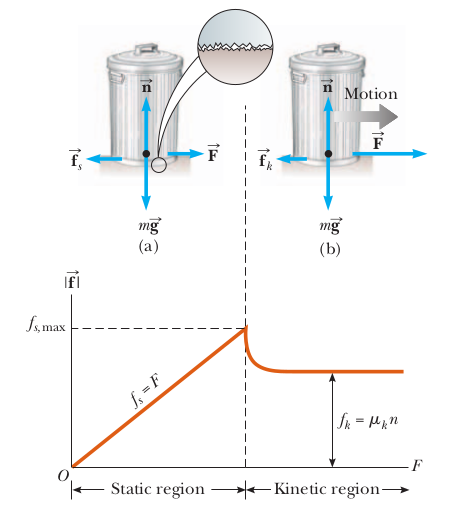
\includegraphics[scale=0.5]{friction.png}

What causes friction? Friction results from the fact that the two surfaces (the ground and the object) are not perfectly smooth. This means that there are hills from one surface that get "stuck" with valleys of the other surface and vice versa. When we try to move the object in a certain direction, the electromagnetic forces between the trapped teeth push backwards in complicated ways, leading to the macroscopic phenomenon of friction.



\section{Specific Examples: Pulley, Massive Rope}
\subsection{Pulley Problems}
Consider the following scenario:
We have a pulley configured in the picture below:


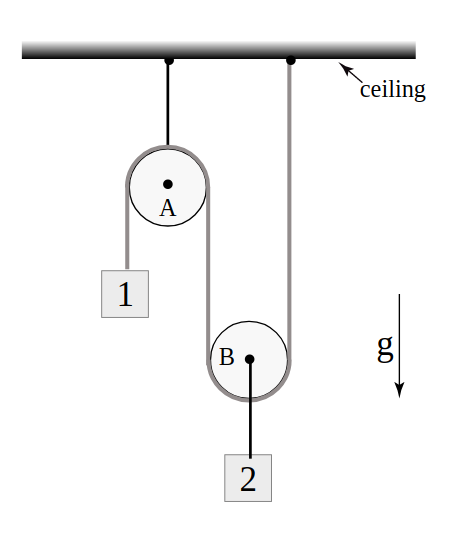
\includegraphics[scale=0.5]{pulley.png}

How can we solve for an expression of their accelerations?

Let's put some labels to things:

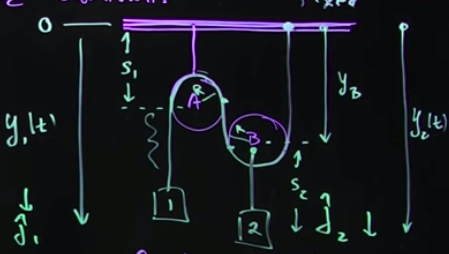
\includegraphics[scale=0.5]{pulley_labels.png}

The total length of the string is then:

$$L = (y_1 - s_1) + \pi R + (y_B-s_1)+\pi R + y_B$$
$$=y_1+2y_B-2s_1+2\pi R$$

We know that the length is constant. So that means that first and second derivative must be 0.

We also know that the only things that can move andare dependent on time in this equation are $y_1$ and $y_B$.

$$\dv[2]{L}{t} = \dv[2]{y_1}{t} + 2\dv[2]{y_B}{t} = 0$$

The second derivative of position is acceleration. Thus we get:


$$
\boxed{
a_1 + 2a_B = 0
}
$$

This gives us a constraint on the accelerations!

We can do the same thing we did here with other more complicated pulley problems as well! First, find an expression for the length of the string, take the second derivative of the expression and set it to 0 to solve for an expression relating the various accelerations.

\subsection{Rope with Mass}
Let's consider a rope with some mass $m$ and length $L$ hanging from the wall:

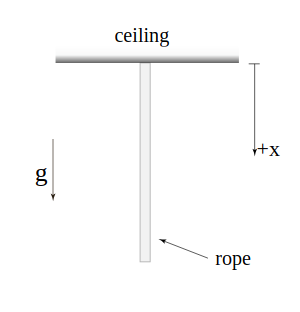
\includegraphics[scale=0.6]{mass_rope.png}

What is the tension at different parts in the rope?

Let's break the rope down into small $\Delta x$:

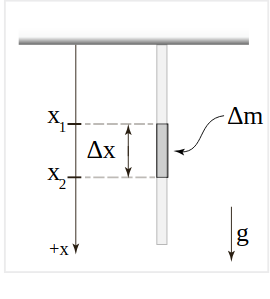
\includegraphics[scale=0.7]{mass_rope_analysis.png}

Each $\Delta x$ segment of the rope has a mass $\Delta m$. Thus, we can analyze the forces in the y direction.

There is a tension force upwards on the small mass element $T(x_1)$ and tension downwards $T(x_1+\Delta x)$. There is also the a gravitational force downwards $\Delta m g$.

Adding the forces together and setting them to 0 (since our system is in equilibrium) gives us:


$$\sum \mathbf{F} = T(x_1)-T(x_1+\Delta x) - \Delta m g = 0$$

Let's introduce a constant called \textbf{mass density}:

$$\mu = \frac{m}{L}$$

Thus,
$$\Delta m = \mu\Delta x$$

Plugging this into our equation and moving terms:
$$T(x_1+\Delta x)-T(x_1) = -\mu\Delta x g $$

Dividing by $\Delta x$:
$$\frac{T(x_1+\Delta x)-T(x_1)}{\Delta x} = -\mu g$$

Let's take the limit as $\Delta x \to 0$:

$$\lim_{\Delta x \to 0}\frac{T(x_1+\Delta x)-T(x_1)}{\Delta x} = -\mu g$$

From calculus, we know the left hand side is just the definition of a derivative:

$$\dv{T(x)}{x} = -\mu g$$

Taking integrals of both sides up to an arbitrary $x$:

$$\int_{T(0)}^{T(x)} \dd T(x) = \int_0^x-\mu g \dd x$$

This is just:

$$T(x) - T(0) = -\mu g x$$


What is $T(0)$?
Since at the top we have to support the entire weight of the rope, the tension must be:

$$T(0) = mg = \mu g L$$

Thus,
$$T(x) = \mu g L- \mu g x$$

$$\boxed{
T(x) = \mu g(L-x)
}$$


\section{Fluid Mechanics}




\chapter{Energy}
\section{Introduction}
Energy plays an enormous role in running almost all processes in the world. It is hard to precisely define what it is and the definition is often circular.



\section{Work}
\subsection{Constant Force}
Let's introduce a new concept called work.

Imagine applying a constant force on some block with some mass. If you applied the force vertically, you would see no movement, no matter what magnitude of the force you applied. 

The work done by you is defined to be:

\begin{mytheo}{Work by Constant Force}{workConst}
    The work done by a constant force on a body is:
    
    $$W = |\mathbf{F}|\Delta r \cos(\theta)$$
    
    where 
    $\mathbf{F}$ - is the force being applied
    $\Delta r$ is the displacement of the object
    $\theta$ is the angle between the object's movement and force being applied
    
    It is measured in $N \vdot m$ or joules(J)
\end{mytheo}

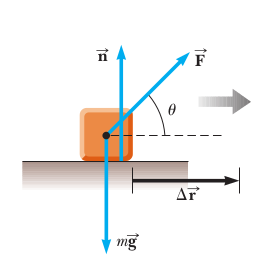
\includegraphics[scale=0.5]{work.png}


Thus, the work done is simply the magnitude of the force in the direction of movement of the object multiplied by the actual movement of the object.


We can use the concept of the dot product to simplify our analysis, since the geometric interpretation of it in fact is the function described above:


\begin{mytheo}{Formula for Work by Constant Force}{workConst}
    The work done by a constant force can also be represented as:
    $$W = |\mathbf{F}|\Delta r \cos(\theta) = \mathbf{F} \vdot \Delta r$$
\end{mytheo}


\subsection{Changing Force}

Imagine that the force is changing as we're moving our object. How do we find the work done by us to move the object?

Let's consider the work done for a tiny distance $\Delta x$. It should be approximately:

$$W(x) \approx \mathbf{F}(x) \vdot \Delta r$$

where $\mathbf{F}$(x) is the force applied at the position $x$.

The total work done by our movement can then be the sum of all of these tiny works:

$$W \approx \sum_{x=x_i}^{x_f}\mathbf{F}(x)\vdot \Delta r$$

As we take smaller and smaller $\Delta r$ we get more and more exact answers and approach an integral:

$$W = \lim_{\Delta r \to 0}\sum_{x=x_i}^{x_f}\mathbf{F}(x)\vdot \Delta r = \int_{x_i}^{x_f}\mathbf{F}(x)\vdot \dd r$$

This process can be understood best visually:

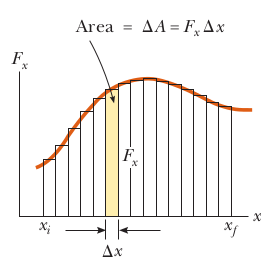
\includegraphics[scale=0.5]{work_area_a.png}
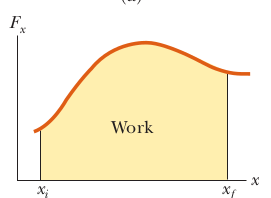
\includegraphics[scale=0.5]{work_area_b.png}

Thus the most general way to calculate work is:

\begin{mytheo}{Work Done by a Changing Force}{workChange}
    The work performed by a force that is changing with distance moving an object from one point $r_i$ to another point $r_f$  is:
    $$W = \int_{r_i}^{r_f} \mathbf{F}(x)\vdot \dd r$$
    
\end{mytheo}
If different forces are acting on the same point mass, we can model the net work performed on the point mass as:


$$ \boxed{
W_{net} = \sum W = \int_{x_i}^{x_f}\sum \mathbf{ F}(x)\vdot \dd r}
$$




\section{Kinetic Energy and Potential Energy}
\section{Conservative vs Non-conservative Forces}
\section{Conservative Forces and Potential Energy}
\section{Conservation of Energy}
\section{Power}
\section{Collisions}


\chapter{Rotational Motion and Rigid Bodies}
\section{Introduction}
\section{Center of Mass}
\section{Angular Velocity and Acceleration}
\section{Moment of Inertia}
\section{Torque}
\section{Angular Momentum}
\section{Torque and Angular Momentum}
\section{Rotating Kinetic Energy}
\section{Rolling}
\section{Gyroscopes}


\chapter{Questions}
\begin{itemize}
    \item Force and energy relationship?
    \item For an object rotating around an origin, what happens when a force is applied perpendicularly in the same plane of the object(i.e. in the direction of Centripetal acceleration)?
    \item For an object rotating around an origin, what happens when a force is applied perpendicularly from outside the plane of the object?
    \item What happens when you apply a force to one point of a rotating object?
    \item How does gyroscopic procession work?
    \item What happens when the torque is in the direction of rotation for a wheel?
    \item Fundamentally, how can an object push another object by just being further away from it using a pulley?
    \item How does the torque caused by gravity on a spinning wheel connected to a rod connected to a string correspond to a change in ?
    \item What is the cause of rotation (i.e. why does applying a force beside the c.m create rotation)?
    \item Is conservation of angular momentum just a byproduct of conservation of momentum?
    \item E\&M Question, at what speed would two electrons need to go for their magnetic field to overtake the electric field?
    \item How is it that when we apply a force off the center of mass of a body, that the center of mass accelerates by the same amount? How is this possible when kinetic energy is being "lost" due to rotation?
    \item Why can we view gravity acting only on the center of mass?
    \item Why does the net torque equal moment of inertia times angular acceleration?
    \item Why does torque due to internal force equal 0?
    \item Why is the angular momentum independent of starting point if sum of linear momentum is 0?
    \item Why does the angular momentum of a rotating symmetric body constant for any point (even outside the axis of symmetry)?
    bcuz angular momentum is constant when linear momentum is constant, which is the case when we have a symmetric body.
    \item Why is the center of mass reference point have all points with momentum 0 for a rotating body?
    \item What is the formula for ang momentum and torque around a rotation and translation around center of mass?
    \item How does friction work?
\end{itemize}



\chapter{Appendix}
\section{\hyperref[th:kin]{Proof of Kinematics Equations}}
\label{sec:kin}

Let's start with the first one.

We know that:

$$a=\dv{v}{t}$$

This is a first order differential equation we can solve:

$$\int{ a \dd t} = \int{ \dd v}$$

At the start an end points
$$a\int_{t_i}^{t_f}{ \dd t} = \int_{v_i}^{v_f}{ \dd v}$$
$$= a \Delta t = v_f - v_i$$

Rearranging we get:

\boxed{
$$v_f - v_i = a \Delta t$$
}


For the second equation, we can use some geometry.

We know that the velocity under constant acceleration is a straight line when plotted with time:

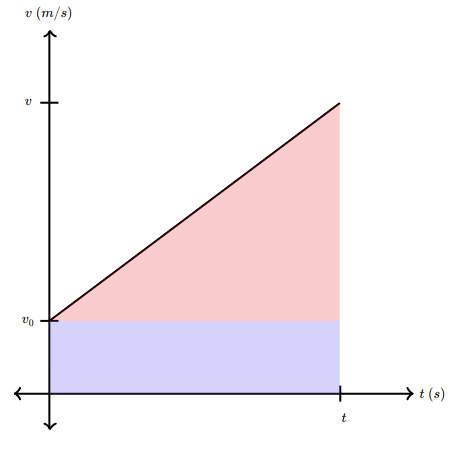
\includegraphics[scale=0.5]{vel_time.png}

The area under the graph is just the sum of the blue rectangle and the red triangle.

By using basic area formulas, we get:

$$\Delta x = v_0t + \frac{1}{2}(v_f-v_i)\Delta t$$
$$= \frac{1}{2}(v_f+2v_i-v_i)\Delta t$$
\boxed{
$$\Delta x = \frac{1}{2}(v_f+v_i)\Delta t$$}

Notice that we could also think about the area of the rectangle plus the triangle as just an area of a bigger rectangle with height $v_f+v_i$!

For the third kinematics equation we can use the triangle also.

The area of the blue rectangle is $v_0 \Delta t$. The area of the red triangle is $\frac{1}{2}(v_f-v_i)\Delta t$

We know that from our first kinematics equation that $v_f -v_i = a\Delta t$.

Plugging this into the area of our red triangle gives us:
$$\frac{1}{2}a(\Delta t)^2$$

The total displacement is just the sum of these individual areas, thus:

\boxed{
$$\Delta x = v_0\Delta t + \frac{1}{2}a(\Delta t)^2$$}

We can also derive this one through calculus by integrating $\dv{x}{t} = v_0 + at$.

To derive the last kinematics equation, let's start with the second one:

$$\Delta x = \frac{1}{2}(v_0+v_f)\Delta t$$

We know from our first equation: 
$$v_f - v_i = a\Delta t$$
Rearranging gives us:
$\Delta t = \frac{v_f-v_i}{a}$

Plugging this back into the equation above gives us:

$$\Delta x = \frac{1}{2}(v_0+v_f)\frac{v_f-v_i}{a}$$
which by simplifying is:

\boxed{
$$v_f^2 - v_i^2 = 2a\Delta x$$}

Which is our last kinematics equation!








\end{document}
